% ============================================================
% MemMark: State-Evolution Attribution Watermarking for
%          Long-Term Agent Memory Systems
%
% Main file. Section bodies live in sections/, tables in
% tables/, figures in figures/. Body text is intentionally
% left as \todo{...} stubs at this stage — only structural
% scaffolding (sections, table/figure environments,
% labels, captions) is filled in.
% ============================================================

\documentclass[11pt]{article}

% Change "review" to "final" for camera-ready, "preprint" for
% non-anonymous with page numbers.
\usepackage[review]{acl}

\newcommand{\decision}{{d}}


\usepackage{times}
\usepackage{latexsym}
\usepackage[T1]{fontenc}
\usepackage[utf8]{inputenc}
\usepackage{microtype}
\usepackage{inconsolata}
\usepackage{graphicx}

% MemMark-specific packages
\usepackage{booktabs}      % \toprule, \midrule, \bottomrule
\usepackage{multirow}      % multi-row table cells
\usepackage{array}         % column type tweaks
\usepackage{amsmath}       % math environments
\usepackage{amssymb}       % math symbols
\usepackage{amsthm}        % theorem environments
\usepackage[dvipsnames]{xcolor}  % colored \todo notes, ForestGreen etc.
\usepackage{enumitem}      % tight list spacing
\usepackage{algorithm}     % algorithm float
\usepackage{algpseudocode} % \State / \If
\usepackage{tikz}          % overview / pipeline diagrams
\usetikzlibrary{arrows.meta,positioning,shapes,fit,calc}
\usepackage[most]{tcolorbox}  % prompt boxes
\usepackage{pifont}        % \checkmark / \xmark
\usepackage{makecell}      % \makecell for table headers
\usepackage{siunitx}       % aligned numeric columns
\sisetup{detect-all,table-format=1.3}

% Inline TODO marker — visible during drafting, removable
% by setting \renewcommand{\todo}[1]{} at submission time.
\newcommand{\todo}[1]{\textcolor{red}{[\textbf{TODO:} #1]}}
\newcommand{\note}[1]{\textcolor{blue}{[\textit{note:} #1]}}

% Theorem environments (used by §3 lemma statements).
\theoremstyle{plain}
\newtheorem{lemma}{Lemma}
\newtheorem{theorem}{Theorem}
\theoremstyle{definition}
\newtheorem{definition}{Definition}

% Symbols used throughout (kept here so they're consistent).

\renewcommand{\decision}{D_t}



\newcommand{\nonceT}{\mathit{nonce}_t}
\newcommand{\carrier}{\mathrm{carrier}}
\newcommand{\candset}{\mathcal{C}}
\newcommand{\probdist}{\pi}
\newcommand{\ctx}{\mathrm{ctx}}
\newcommand{\commit}{\mathrm{cm}}
\newcommand{\header}{\mathrm{hdr}}
\newcommand{\reveal}{\mathrm{rev}}
\usepackage[table]{xcolor}
\definecolor{cbblue}{RGB}{198,219,239}   
\newcommand{\best}[1]{\cellcolor{cbblue}#1}
\newcommand{\bitsperdec}{\textsc{bpd}}

% Backend name styling.
\newcommand{\amem}{\textsc{A-Mem}}
\newcommand{\graphiti}{\textsc{Graphiti}}
\newcommand{\memmark}{\textsc{MemMark}}
\newcommand{\agentmark}{\textsc{AgentMark}}
\newcommand{\kgmark}{\textsc{KGMark}}
\newcommand{\tiermem}{\textsc{TierMem}}
\newcommand{\locomo}{LoCoMo}
\newcommand{\longmemeval}{LongMemEval}
\newcommand{\mab}{MemoryAgentBench}

% =================== title / authors ===================
\title{\memmark: State-Evolution Attribution Watermarking for Long-Term Agent Memory Systems}

\author{
  Anonymous Authors \\
  Anonymous Affiliation \\
  \texttt{anon@example.org} \\
}

\begin{document}
\maketitle

% =================== body ===================
% ============================================================
% Abstract — three pillars: (1) the watermark mechanism,
% (2) R3 attribution headline, (3) utility preservation.
% ============================================================

\begin{abstract}
\todo{Field-stamping provenance (TierMem, MemOS, enterprise
tagging) assumes the writer is honest, but in the most
forensically valuable setting — a memory snapshot leaks, is
distilled, or migrates across systems — the holder of the snapshot
\emph{is} the writer. Token-level and action-layer watermarks
likewise fail because the original output text and action
trajectory are gone before the memory leaves the system. We
present \memmark{}, a watermark for long-term agent memory
systems that embeds attribution into the memory backend's own
latent evolve decisions: at each internal LLM call we elicit $K$
equivalent candidates with self-reported weights, then keyed-pick
via the distribution-preserving \agentmark{} binning sampler. Each
selection is committed into a Merkle log whose signed anchor and
per-leaf inclusion proofs are co-located with the memory record
itself. On \locomo{} across \amem{} and \graphiti{}, \memmark{}
(i) \textbf{preserves utility} on F1 / BLEU-1 / ROUGE-L within
statistical noise of the unwatermarked baseline; (ii) achieves
\textbf{R3 (snapshot-only) bit\_recovery $= 1.00$} versus $0$ for
a \texttt{signed-metadata-only} baseline and $0.15$ for the
wrong-key control — the central claim of the paper; (iii) remains
\textbf{robust} under nine memory-lifecycle attacks. Code, audit
traces, and benchmarks are released.}
\end{abstract}

% ============================================================
% Introduction — README §1
%   §1.1 Provenance-aware memory is a hot topic, bound to honest writers
%   §1.2 But the attacker is the writer
%   §1.3 Attribution as behavioral trace, not field
%   §1.4 Headline: In-Record Attribution Verification (R3)
%   §1.5 Contributions
% ============================================================
\section{Introduction}
\label{sec:intro}

% ---------- §1.1 honest-writer premise ----------
\paragraph{Provenance-aware memory is bound to honest writers.}
\todo{Open with the active line of work (\tiermem, MemOS MemCube,
enterprise stamping) and the structural assumption they share:
metadata fields are facts because the writer is trusted. Cite
\tiermem{} and MemOS preprints. End with the failure mode: once
memory leaves the original system, that assumption collapses.}

% ---------- §1.2 attacker is the writer ----------
\paragraph{The attacker is the writer.}
\todo{Enumerate what the snapshot-holder can do: stamp ownership,
erase \texttt{source\_agent} / \texttt{tenant\_id}, fabricate
provenance chains, rewrite the memory system's own changelog
(\amem{} evolve history, \graphiti{} fact-invalidation chain) since
they sit in the same store. Conclude: any field-based provenance is
ill-defined in adversarial storage. Token-level LLM watermarks and
agent action-layer watermarks don't fill the gap — they assume the
trajectory survives, which it doesn't in the most forensically
valuable case.}

% ---------- §1.3 attribution = behavioral trace ----------
\paragraph{Attribution as behavioral trace, not field.}
\todo{Frame the three carriers (update / link / semantic) as latent
decisions every memory write makes. Properties: (i) non-trivial
candidate space, (ii) equivalent choices don't break utility, (iii)
the choice itself is readable from the snapshot. Then embed a PRF
key into the sequence of keyed picks: $\nonceT = \text{PRF}(K, \ctx)$
selects which equivalent candidate is realized. Reads as ``\emph{the
writer's key can be replayed against the snapshot}'' rather than
``\emph{we say so}''.}

% ---------- §1.4 R3 headline ----------
\paragraph{In-Record Attribution Verification (R3).}
\todo{Define the three regimes R1 (full external log) / R2 (partial
log) / R3 (snapshot only). R3 is the headline: bind each keyed
selection into a per-decision commitment, anchor the per-session
Merkle root + signature directly inside the snapshot, and store the
reveal record co-located with the memory record itself. Forward to
\S\ref{sec:rq3} for the numbers.}

% ---------- §1.5 contributions (3 pillars) ----------
% Three threads of the paper:
%   (i)   The watermark mechanism (carrier taxonomy + interception
%         + keyed sampling + cryptographic audit trace, packaged as
%         one engineering contribution).
%   (ii)  In-Record Attribution Verification (R3), the headline
%         result that no prior watermark or provenance scheme
%         provides under adversarial storage.
%   (iii) Memory-specific evaluation showing utility preservation
%         within statistical noise + robustness under 9 attacks.
\paragraph{Contributions.}
\begin{enumerate}[topsep=2pt,itemsep=2pt,leftmargin=*]
\item \textbf{A watermark for long-term agent memory.}
  \todo{One sentence on the end-to-end mechanism: backend-invariant
  $\langle \carrier, \candset, \probdist, \ctx \rangle$ taxonomy
  (\S\ref{sec:method-formal}), \agentmark-style 1-call enumeration
  that produces $(\candset, \probdist)$ from open-vocabulary
  structured-JSON LLM output (\S\ref{sec:method-interception}),
  distribution-preserving keyed sampling on the SDK's internal LLM
  calls (\S\ref{sec:method-sampler}), and a cryptographic audit
  trace (commitment + per-session Merkle log + signed in-snapshot
  anchor + per-leaf inclusion proof; \S\ref{sec:method-audit})
  that supports snapshot-only verification.}
\item \textbf{In-Record Attribution Verification (R3).}
  \todo{One sentence on the three-regime hierarchy and the
  empirical result: \memmark{} recovers the full payload from
  snapshot alone with bit\_recovery $= 1.00$ on \locomo{}, while
  a \texttt{signed-metadata-only} baseline drops to $0$ and the
  wrong-key control drops to $0.15$ (\S\ref{sec:rq3}). No prior
  watermark or provenance scheme provides snapshot-only attribution
  under the adversarial-storage threat model.}
\item \textbf{Memory-specific evaluation across two backends and
  two LLMs.} \todo{One sentence: utility preserved within
  statistical noise on \locomo{} (\S\ref{sec:rq1}); non-trivial
  capacity (\S\ref{sec:rq2}); robust under nine memory-lifecycle
  attacks including KGMark-style edge relabel and subgraph
  reanchor (\S\ref{sec:rq4}); ingestion integrity unaffected
  (\S\ref{sec:rq5}).}
\end{enumerate}

% ---------- pointer figure ----------
% ============================================================
% Figure: Overview of MemMark's storyline (3-panel)
%   panel A: provenance-as-field (attacker forges)
%   panel B: keyed-decision behavioral trace (attacker can't forge)
%   panel C: R3 in-record verification (snapshot-only)
% ============================================================
\begin{figure*}[t]
\centering
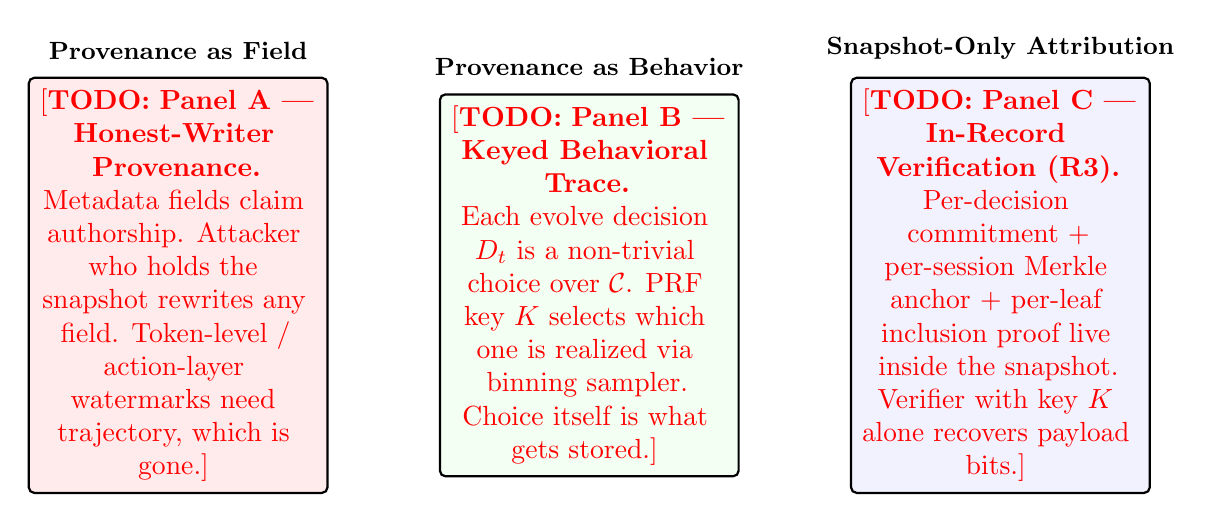
\begin{tikzpicture}[
  node distance=8mm and 14mm,
  panel/.style={draw, thick, rounded corners=2pt, minimum width=0.30\textwidth, minimum height=4.2cm, align=center, inner sep=4pt},
  attacker/.style={fill=red!8},
  honest/.style={fill=green!5},
  reader/.style={fill=blue!5},
  title/.style={font=\bfseries\small},
]

% Panel A — honest writer assumption
\node[panel, attacker] (A) {
  \begin{minipage}{0.28\textwidth}
  \centering
  \todo{\textbf{Panel A — Honest-Writer Provenance.}\\
  Metadata fields claim authorship. Attacker who holds the
  snapshot rewrites any field. Token-level / action-layer
  watermarks need trajectory, which is gone.}
  \end{minipage}
};

% Panel B — keyed behavioral trace
\node[panel, honest, right=of A] (B) {
  \begin{minipage}{0.28\textwidth}
  \centering
  \todo{\textbf{Panel B — Keyed Behavioral Trace.}\\
  Each evolve decision $\decision$ is a non-trivial choice over
  $\candset$. PRF key $K$ selects which one is realized via
  binning sampler. Choice itself is what gets stored.}
  \end{minipage}
};

% Panel C — R3 in-record verification
\node[panel, reader, right=of B] (C) {
  \begin{minipage}{0.28\textwidth}
  \centering
  \todo{\textbf{Panel C — In-Record Verification (R3).}\\
  Per-decision commitment + per-session Merkle anchor + per-leaf
  inclusion proof live inside the snapshot. Verifier with key
  $K$ alone recovers payload bits.}
  \end{minipage}
};

% Title labels above
\node[title, above=1mm of A] {\textsc{Provenance as Field}};
\node[title, above=1mm of B] {\textsc{Provenance as Behavior}};
\node[title, above=1mm of C] {\textsc{Snapshot-Only Attribution}};

\end{tikzpicture}
\caption{\textbf{\memmark{} in three panels.} (A) Field-based
provenance assumes the writer is honest; once the attacker holds
the snapshot, all fields are writable. (B) \memmark{} embeds
attribution into the memory system's own latent evolve decisions
via a PRF-keyed binning sampler that preserves the marginal
$\probdist$ distribution per Lemma~\ref{lem:dist-preserve}. (C) The
in-record audit trace (commitment + Merkle anchor + per-leaf
inclusion proof) lets a verifier with only the snapshot and key
$K$ decode the writer's bits — RQ3 headline.}
\label{fig:overview}
\end{figure*}


% ============================================================
% Related Work — main paper keeps only the two CLOSEST lines:
%   §2.1 Agent behavioral watermarking (mechanism-adjacent)
%   §2.2 Long-term memory systems + provenance (problem-adjacent)
% Everything else (RAG/corpus, LLM text, crypto primitives,
% memory-ops-as-actions extras) → Appendix \ref{app:related-ext}.
% ============================================================
\section{Related Work}
\label{sec:related}

\todo{One-sentence lede: \memmark{} sits at the intersection of two
research lines — behavioral watermarking for LLM agents (which gives
us the mechanism) and long-term memory systems with provenance
(which gives us the threat model). Extended coverage of RAG /
corpus-level watermarking, LLM text watermarking, and cryptographic
provenance primitives is deferred to
Appendix~\ref{app:related-ext}.}

% ============================================================
\subsection{Behavioral Watermarking for LLM Agents}
\label{sec:related-behavioral}
% ============================================================
\todo{Cite \agentmark~\cite{agentmark}, Agent
Guide~\cite{agentguide}, ActHook~\cite{acthook},
AGENTWM~\cite{agentwm}. All four embed at the visible-action layer
(planning, tool call, trajectory) and require the trajectory at
verify time. \memmark{} embeds at the latent state-evolution
decision layer, which survives when the trajectory is gone.}

\todo{Relation to \agentmark: we reuse its binning sampler as a
black-box component inside \S\ref{sec:method-sampler}; the
contribution is not the sampler but (a) where to intercept inside a
third-party memory SDK, (b) how to construct $(\candset, \probdist)$
from open-vocabulary structured-JSON LLM output, and (c) how to
compose audits across a cascade of intercepted calls per memory
event.}

\todo{Adjacent line — memory ops as actions
(\textsc{Memory-as-Action}~\cite{mem-as-action},
A-MAC~\cite{a-mac}). These optimize \emph{which} memory op to take;
\memmark{} embeds attribution \emph{into} the op. Orthogonal but
the closest neighbor on the "memory writes are first-class
decisions" axis.}

% ============================================================
\subsection{Long-Term Memory Systems and Provenance}
\label{sec:related-memory}
% ============================================================
\todo{Operating environment: \amem~\cite{amem},
\graphiti~\cite{graphiti}, MemOS~\cite{memos},
MemMachine~\cite{memmachine}. Two are the backends we wrap
(\amem{} agentic notes, \graphiti{} temporal graph); the other two
are MemMark-compatible via the §\ref{sec:method-formal} adapter.}

\todo{Provenance-aware designs:
\tiermem~\cite{tiermem} ships explicit provenance chains and
immutable source anchoring; MemOS \texttt{MemCube} carries
versioning / origin / lifecycle fields. Both are
\emph{field-stamping} provenance — they encode "who wrote this"
into metadata that the writer controls. \memmark{}'s contrast is
exactly this: we treat the snapshot-holder as the writer (adversarial
storage), so any field-based provenance is forgeable. \tiermem{} /
MemOS therefore appear in \S\ref{sec:rq3} as the
\texttt{signed-metadata-only} ablation point.}

\todo{Threat-side motivation: A-MemGuard~\cite{amemguard} and
MemoryGraft~\cite{memorygraft} catalog memory-poisoning attacks on
LLM agents — these motivate our \S\ref{sec:rq4} attack model
(\texttt{poisoning}, \texttt{manual\_edits}). The Mnemonic
Sovereignty survey~\cite{mnemonicsovereignty} covers governance /
access control / poisoning defense but explicitly does not cover
behavioral watermarking on memory-evolve decisions, supporting our
positioning.}

\todo{Direct KG-backend baseline: \kgmark~\cite{kgmark} is dynamic
knowledge-graph watermarking and is the closest single-point
comparison on KG-structured memory. \S\ref{sec:rq1}–\S\ref{sec:rq4}
compare \memmark{} vs \kgmark{} on the \graphiti{} backend.
\kgmark{} is not applicable to \amem{} (notes network, not strict
KG).}

% ---------- positioning table (stays in main paper) ----------
% ============================================================
% Table: Related Work positioning matrix (README §10.6)
% ============================================================
\begin{table*}[t]
\centering
\small
\setlength{\tabcolsep}{4pt}
\renewcommand{\arraystretch}{1.15}
\newcommand{\yes}{\textcolor{ForestGreen!80!black}{\checkmark}}
\newcommand{\no}{\textcolor{red!70!black}{\ding{55}}}
\newcommand{\partial}{$\circ$}
\begin{tabular}{lcccccc}
\toprule
Dimension &
\makecell{Agent Behavioral\\(\agentmark{}, etc.)} &
\makecell{RAG / Corpus\\(RAG-WM, etc.)} &
\makecell{\kgmark{}\\(KG-only)} &
\makecell{LLM Text\\(KGW, etc.)} &
\makecell{Memory Systems\\(\tiermem, MemOS)} &
\textbf{\memmark} \\
\midrule
Behavioral (vs static)        & \yes & \no  & \yes & \no  & N/A & \yes \\
Embedded in memory layer      & \no  & \no  & \yes & \no  & N/A & \yes \\
In-record verifiable (no ext.\ log) & \no  & \no  & \no  & \no  & partial & \yes \\
Robust to memory lifecycle    & \no  & partial & partial & \no  & N/A & \yes \\
Cryptographic audit           & \no  & \no  & \no  & \no  & metadata only & \yes \\
Backend-invariant             & N/A  & partial & \no  & N/A  & N/A & \yes \\
\bottomrule
\end{tabular}
\caption{\textbf{Positioning matrix}. No prior line simultaneously
covers behavioral $\times$ memory-layer $\times$ in-record
verification $\times$ lifecycle robust $\times$ cryptographic audit
$\times$ backend-invariant. \kgmark{} and \tiermem{} are the two
closest neighbors; \memmark{} integrates the keyed-sampling stance
of one with the provenance-aware stance of the other across three
structurally different memory backends. \emph{partial} = supported
only under restrictive assumptions; see \S\ref{sec:related} per-cell
discussion.}
\label{tab:related-positioning}
\end{table*}


% ============================================================
% Method — README §3, §6, §7, §8
%   3.1 Problem formalization + carrier taxonomy (§3.2)
%   3.2 LLM-call boundary interception (§6.1)
%   3.3 Self-reported candidate sampling (§6.2 / §6.3)
%   3.4 Cryptographic audit trace (§8)
% ============================================================
\section{Method}
\label{sec:method}

% ---------- pipeline figure ----------
% ============================================================
% Figure: End-to-end MemMark pipeline (data flow diagram)
% ============================================================
\begin{figure*}[t]
\centering
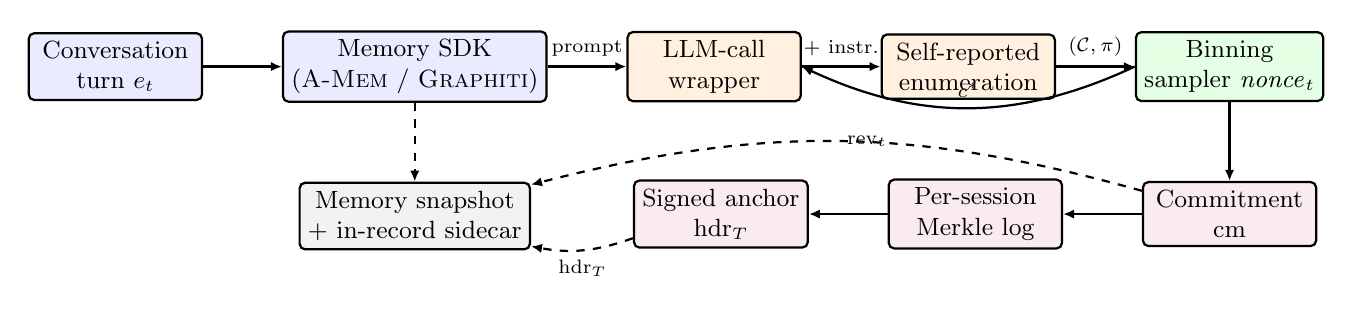
\begin{tikzpicture}[
  node distance=6mm and 10mm,
  block/.style={draw, thick, rounded corners=2pt, minimum height=8mm, minimum width=22mm, align=center, font=\small, inner sep=3pt},
  sdk/.style={block, fill=blue!8},
  wrapper/.style={block, fill=orange!12},
  sampler/.style={block, fill=green!10},
  store/.style={block, fill=gray!10},
  audit/.style={block, fill=purple!8},
  flow/.style={-{Latex[length=1.4mm,width=1.2mm]}, thick},
  flowdash/.style={-{Latex[length=1.4mm,width=1.2mm]}, thick, dashed},
]

% Top row: ingestion path
\node[sdk] (event) {Conversation\\turn $e_t$};
\node[sdk, right=of event] (backend) {Memory SDK\\(\amem{} / \graphiti{})};
\node[wrapper, right=of backend] (wrap) {LLM-call\\wrapper};
\node[wrapper, right=of wrap] (enum) {Self-reported\\enumeration};
\node[sampler, right=of enum] (samp) {Binning\\sampler $\nonceT$};
\node[audit, below=10mm of samp] (commit) {Commitment\\$\commit$};
\node[audit, left=of commit] (merkle) {Per-session\\Merkle log};
\node[audit, left=of merkle] (anchor) {Signed anchor\\$\header_{T}$};

% Storage
\node[store, below=10mm of backend] (store) {Memory snapshot\\+ in-record sidecar};

% Top-row flow
\draw[flow] (event) -- (backend);
\draw[flow] (backend) -- node[above,font=\scriptsize]{prompt} (wrap);
\draw[flow] (wrap) -- node[above,font=\scriptsize]{+ instr.} (enum);
\draw[flow] (enum) -- node[above,font=\scriptsize]{$(\candset, \probdist)$} (samp);
\draw[flow] (samp.west) to[bend left=25] node[above,font=\scriptsize]{$c^*$} (wrap.east);

% Audit flow
\draw[flow] (samp) -- (commit);
\draw[flow] (commit) -- (merkle);
\draw[flow] (merkle) -- (anchor);

% Persistence
\draw[flowdash] (backend) -- (store);
\draw[flowdash] (commit) to[bend right=15] node[right,font=\scriptsize]{$\reveal_{t}$} (store);
\draw[flowdash] (anchor) to[bend left=15] node[below,font=\scriptsize]{$\header_T$} (store);

\end{tikzpicture}
\caption{\textbf{End-to-end \memmark{} pipeline.} The memory SDK
issues an internal LLM call (blue). Our wrapper (orange) appends an
\agentmark-style enumeration instruction; the LLM self-reports
$K$ alternatives with weights $(\candset, \probdist)$. The binning
sampler (green) keyed-picks $c^*$ via $\nonceT = \text{PRF}(K,
\ctx)$. Each pick produces a commitment, gets appended to the
per-session Merkle log, and contributes to the signed anchor
$\header_T$ (purple). At seal time the anchor and the reveal record
land directly inside the memory snapshot, enabling R3 in-record
verification without any external audit store.}
\label{fig:pipeline}
\end{figure*}


% ============================================================
\subsection{Problem Formalization and Carrier Taxonomy}
\label{sec:method-formal}
% ============================================================
\todo{Define memory state $M_t$, incoming event $e_t$, evolve
decision $\decision = \langle \carrier, \candset, \probdist, \ctx
\rangle$ with $\carrier \in \{\text{update}, \text{link},
\text{semantic}\}$. State the backend-invariance: \memmark{} reads
only $(\candset, \probdist, \ctx)$, never touches backend internals.
Match \S3.2 of the README. Include a table summarizing the three
carriers across \amem{} / \graphiti{}.}

% ============================================================
% Table: 3 carriers across A-Mem / Graphiti
% Lives in §3.1 Method.
% ============================================================
\begin{table}[t]
\centering
\small
\setlength{\tabcolsep}{4pt}
\begin{tabular}{lll}
\toprule
Carrier $\carrier$ & \amem{} instance & \graphiti{} instance \\
\midrule
\texttt{update\_target}
  & note id (which to update)
  & fact-edge id / episode \\
\texttt{link\_target}
  & keyword cluster / tag
  & entity attach point \\
\texttt{semantic\_realization}
  & note description + tags
  & edge label / fact phrasing \\
\bottomrule
\end{tabular}
\caption{\textbf{Three carriers, two backends}. Each $\carrier$ is a
non-trivial-candidate-set evolve decision realized in
backend-specific form; the watermark sampler reads only
$(\candset, \probdist, \ctx)$ and is therefore backend-invariant.}
\label{tab:carrier-taxonomy}
\end{table}


\todo{Then list the minimum adapter signature
($\texttt{enumerate\_candidates}$, $\texttt{score\_candidates}$,
$\texttt{apply\_selected}$) and the per-carrier reportable quantities
($|\candset|$, $H(\probdist)$, acceptance rate).}

% ============================================================
\subsection{LLM-Call Boundary Interception}
\label{sec:method-interception}
% ============================================================
\todo{Key observation: each SDK-internal LLM call is itself an
$\varepsilon$-equivalent decision point at $T{=}0.7$. We hot-swap
the SDK's LLM client with a wrapper (\amem{}: replace
\texttt{AgenticMemorySystem.llm\_controller}; \graphiti{}: replace
\texttt{Graphiti.llm\_client}). Wrapper appends an \agentmark-style
instruction to the SDK's prompt asking the LLM to enumerate $K$
alternatives with self-reported weights in a single call. The wrapper
parses, runs keyed pick via the binning sampler, returns the chosen
decision in the SDK's expected schema. Backend doesn't know.}

% prompt template figure
% ============================================================
% Figure: AgentMark-style prompt instruction (verbatim)
% ============================================================
\begin{figure}[t]
\centering
\begin{tcbox}[colback=gray!4, colframe=black!50, fontupper=\ttfamily\scriptsize, width=0.97\linewidth, boxsep=2pt, left=2pt, right=2pt, top=2pt, bottom=2pt]
CRITICAL OVERRIDE: instead of returning a single answer, return JSON in EXACTLY this multi-candidate form:\\[2pt]
\{\\
\hspace*{1em}"candidates": [\\
\hspace*{2em}\{"decision": <answer matching the original schema>, "weight": <float>\},\\
\hspace*{2em}\{"decision": <plausible alternative>, "weight": <float>\},\\
\hspace*{2em}...\\
\hspace*{1em}],\\
\hspace*{1em}"thought": "..."\\
\}\\[2pt]
- Provide K candidate alternatives;\\
- Each "decision" must independently match the original schema;\\
- Weights $>$ 0, rank by your real preference; sum normalized.
\end{tcbox}
\caption{\textbf{Open-vocabulary $\to$ discrete enumeration prompt.}
Appended verbatim to the memory SDK's original prompt.  Reduces an
unbounded structured-JSON output to a finite candidate set
$(\candset, \probdist)$ via the LLM's self-reported preference
weights. Single call, $K{=}4$ default. Non-compliant return
(weights missing / $|\candset|{<}2$) falls back to a fresh
single-answer call that bypasses sampling and does not log an audit.}
\label{fig:prompt-template}
\end{figure}


% ============================================================
\subsection{Self-Reported Candidate Sampling}
\label{sec:method-sampler}
% ============================================================
\todo{Parse JSON into $(\text{decisions}, \text{weights})$, normalize
weights to $\probdist$, feed to \agentmark's binning sampler with
keyed context $\ctx \| \nonceT$ where $\nonceT = \text{PRF}(K,
\ctx)$. The sampler returns the keyed pick $c^*$ and embedded bits.
Algorithm \ref{alg:sample} sketches the per-call flow.}

% ============================================================
% Algorithm: per-call keyed sample
% ============================================================
\begin{algorithm}[t]
\caption{Watermarked LLM call (per-decision)}
\label{alg:sample}
\begin{algorithmic}[1]
\Require Original SDK prompt $P$; backend LLM client $L$; PRF key $K$;
target candidate count $K_{\text{cands}}{=}4$; context payload $\ctx$
\Ensure SDK-schema-conformant string $c^*$; audit record $\reveal_t$
\Statex
\State $P' \gets P \,\|\, \textsc{AgentMarkInstruction}(K_{\text{cands}})$
\State $\text{raw} \gets L.\text{complete}(P')$ \Comment{1 call, $T{=}0.7$}
\State $(\text{decisions}, \text{weights}) \gets \textsc{ParseJSON}(\text{raw})$
\If{$|\text{decisions}| < 2$ \textbf{or} $\text{weights missing}$}
  \State \Return $L.\text{complete}(P)$ \Comment{passthrough, no audit}
\EndIf
\State $\probdist \gets \textsc{Normalize}(\text{weights})$
\State $\nonceT \gets \text{PRF}(K, \ctx)$
\State $c^* \gets \textsc{BinningSample}(\text{decisions}, \probdist, \nonceT)$
\State $\commit \gets H(\ctx \| H(\candset) \| H(\probdist) \| \text{idx}(c^*) \| \text{bits} \| \nonceT)$
\State $\textsc{MerkleLog}.\text{append}(\commit)$
\State $\reveal_t \gets \{\candset, \probdist, c^*, \nonceT, \ctx\}$
\State \Return $(c^*, \reveal_t)$
\end{algorithmic}
\end{algorithm}


\paragraph{Properties.} \todo{State Lemma 1 (strict
distribution preservation), Lemma 2 (composition across the cascade),
Lemma 3 (backend-invariant marginal). Full proofs in
Appendix~\ref{app:proofs}.}

\begin{lemma}[Strict distribution preservation]
\label{lem:dist-preserve}
\todo{Given $\probdist$, the keyed pick $c^*$ under PRF key $K$ has
marginal distribution equal to $\probdist$: $\Pr[c^* = c_i \mid K,
\ctx]_{\mathrm{marg}} = \probdist(c_i)$.}
\end{lemma}

\begin{lemma}[Cascade composition]
\label{lem:cascade}
\todo{$K$ LLM calls within a memory event yield independent keyed
picks. Capacity is additive in $K$, marginal bias does not
accumulate.}
\end{lemma}

\begin{lemma}[Backend-invariant marginal]
\label{lem:backend-invariant}
\todo{Lemma \ref{lem:dist-preserve} depends only on $\probdist$ and
$K$, not the backend.}
\end{lemma}

% ============================================================
\subsection{Cryptographic Audit Trace}
\label{sec:method-audit}
% ============================================================
\todo{Three-layer design: per-decision commitment, per-session
Merkle log, signed root anchor written into the snapshot itself.
$\commit = H(\ctx \| H(\candset) \| H(\probdist) \| \text{selected}
\| \text{bits} \| \nonceT)$. $\header_T = (\text{agent\_id},
\text{user\_id}, \text{session\_id}, T, \text{root}_T,
\text{sig}_K(\text{root}_T))$.}

\paragraph{Per-leaf inclusion proofs.}
\todo{Each \texttt{AuditRecord} stores its Merkle inclusion path at
seal time so the verifier can check each leaf independently against
$\text{root}_T$ — no rebuilt-root match required. This gives smooth
bit-recovery under structural attacks (pruning / dedup / poisoning),
in contrast to rebuilt-root verification which binary-collapses when
the leaf set changes (see Table~\ref{tab:robustness}).}

\paragraph{Verification regimes.}
\todo{Define R1 (full external log), R2 (partial external log), R3
(snapshot only). Forward to \S\ref{sec:rq3} for the empirical
hierarchy and to Table~\ref{tab:verification} for the regime
matrix.}

% ============================================================
% Experiments — README §9
%   §9.1 Setup
%   §9.2 Metrics (no body, just pointer to table)
%   §9.3 RQ1 Utility
%   §9.4 RQ2 Capacity
%   §9.5 RQ3 In-Record / Snapshot-Only Verification (HEADLINE)
%   §9.6 RQ4 Robustness
%   §9.7 RQ5 Integrity
%   §9.8 RQ6 Composability (appendix-only)
% ============================================================
\section{Experiments}
\label{sec:exp}

% ============================================================
\subsection{Setup}
\label{sec:setup}
% ============================================================
\todo{Backends: \amem{} (agentic notes) and \graphiti{} (temporal
graph). Each via \S\ref{sec:method-formal}'s minimal adapter, no
agent harness. LLMs: \textsc{DeepSeek v4 Pro} (headline + cost) and
\textsc{Qwen3.5-397B-A17B} (open weights + reproducibility), both
OpenAI-compatible, $T_{\text{enum}}{=}0.7$, $T_{\text{score}}{=}0.0$,
JSON mode on. Benchmarks: \locomo{} / \longmemeval{} / \mab{}. F1
follows \amem{} \texttt{utils.py:135--145} set-based formula for
paper-comparability to \amem{} Table 1. $\geq 3$ seeds per
(backend, LLM, benchmark) triple.}

\paragraph{Baselines.} \todo{(1) \texttt{no-watermark} — upper
utility bound. (2) \texttt{random-replace} — FPR / wrong-key floor.
(3) \texttt{signed-metadata-only} — same audit trace, no keyed bit
embedding; isolates marginal value of watermark over pure metadata
in R3. (4) \kgmark{} @ \graphiti{} — direct KG baseline (N/A on
\amem). (5) Action-layer watermark @ ToolBench — cross-layer R1/R2/R3
comparison.}

% Metric definitions table
% ============================================================
% Table: Metric definitions (README §9.2)
% ============================================================
\begin{table*}[t]
\centering
\small
\setlength{\tabcolsep}{3.5pt}
\begin{tabular}{p{0.17\linewidth}p{0.29\linewidth}p{0.46\linewidth}}
\toprule
Category & Metric & Definition / Reporting Unit \\
\midrule

Utility
  & \locomo{} F1
  & precision and recall are computed over predicted versus gold answer
    items, and combined as their harmonic mean. \\

  & BLEU-1
  & Unigram precision between the generated answer and the reference
    answer, measuring lexical overlap at the token level. \\

\midrule

Capacity
  & Bits per memory decision
  & Average number of recoverable watermark bits carried by one write,
    update, delete, link, or merge decision. \\

  & Bits per session
  & Total recoverable watermark capacity within one complete conversation
    session. \\

  & Bits per benchmark episode
  & Total recoverable watermark capacity within one benchmark instance. \\

  & Bits per 100 conversation turns
  & Normalized capacity over long-horizon conversations, reported per
    100 turns. \\

  & Average bits per memory write
  & Average number of recoverable bits carried by each committed memory
    write. \\

\midrule

Carrier-level analysis
  & Per-carrier reliability and capacity
  & All watermark reliability and capacity metrics are additionally
    reported for each carrier:
    $\carrier \in
    \{\text{update\_target}, \text{link\_target},
    \text{semantic\_realization}\}$. \\

\midrule

Robustness
  & Commitment verification fail rate
  & Fraction of tampered memory records whose commitment verification
    fails under the anchored commitment root. Reported per attack type
    in \S\ref{sec:rq4}. \\

  & Merkle proof verification fail rate
  & Fraction of tampered memory records whose Merkle inclusion proof fails
    against the anchored Merkle root. Reported per attack type in
    \S\ref{sec:rq4}. \\

\midrule

Memory integrity
  & Snapshot size
  & Total size of the memory snapshot after watermarking and commitment
    construction. \\

  & Carrier distribution
  & Distribution of embedded bits across carriers, reported overall and
    per $\carrier$. \\

  & Evidence-grounded retrieval recall
  & Fraction of QA-time gold evidence records successfully retrieved from
    memory. \\

  & Write failures
  & Number or fraction of attempted memory writes that fail validation,
    storage, or commitment construction. \\

\bottomrule
\end{tabular}
\caption{Metric definitions across the five research questions. Utility
metrics measure answer quality on \locomo{}; watermark metrics measure
decodability, reliability, and security; capacity metrics quantify how many
bits can be carried by memory operations; carrier-level metrics decompose
performance by watermark carrier; tamper-detection metrics measure whether
memory modifications are caught by commitment and Merkle verification; and
memory-integrity metrics measure the operational side effects of watermarking.
For paper-comparability, F1 follows \amem{}'s set-based formula.}
\label{tab:metric-defs}
\end{table*}

% ============================================================
\subsection{RQ1 — Utility Preservation}
\label{sec:rq1}
% ============================================================
\todo{Question: does watermark embedding break memory system
utility? Setup: \texttt{no-watermark} vs \texttt{+ watermark} on F1
/ BLEU-1 / ROUGE-L (set-based). Result: $\Delta$F1 within statistical
noise across all (LLM, backend, benchmark) triples; retrieve /
generation latency increase $\leq 5\%$; no extra write failures.
Lead with Table~\ref{tab:main-results}, point at
Figure~\ref{fig:per-category} for per-category breakdown.}

% Add to preamble:
% \usepackage[table]{xcolor}
% \newcommand{\best}[1]{\cellcolor{green!18}#1}

\begin{table*}[t]
  \centering
  \scriptsize
  \setlength{\tabcolsep}{3pt}
  \resizebox{\textwidth}{!}{%
  \begin{tabular}{lllcccccccccccc}
  \toprule
  & & & \multicolumn{2}{c}{Single Hop (1)} & \multicolumn{2}{c}{Temporal (2)} & \multicolumn{2}{c}{Multi Hop (3)} & \multicolumn{2}{c}{Open Domain (4)} & \multicolumn{2}{c}{Adversarial (5)} & \multicolumn{2}{c}{\textbf{Overall}} \\
  \cmidrule(lr){4-5}\cmidrule(lr){6-7}\cmidrule(lr){8-9}\cmidrule(lr){10-11}\cmidrule(lr){12-13}\cmidrule(lr){14-15}
  Model & Backend & Method & F1 & BLEU & F1 & BLEU & F1 & BLEU & F1 & BLEU & F1 & BLEU & F1 & BLEU \\
  \midrule
  \multirow{9}{*}{Qwen3.6-Flash}
    & \multirow{4}{*}{A-MEM} & \texttt{No-WM}     & 0.1974 & 0.2373 & 0.3732 & 0.5360 & 0.1363 & 0.2333 & 0.4107 & 0.4265 & 0.1289 & 0.1234 & 0.2850 & 0.3322 \\
    &                         & \texttt{S.M.-Only} & 0.2127 & 0.2682 & \best{0.4727} & \best{0.5676} & 0.1884 & 0.3295 & 0.4115 & 0.4278 & \best{0.2251} & \best{0.2072} & \best{0.3323} & \best{0.3696} \\
    &                         & \texttt{Ran.}      & 0.2305 & \best{0.3364} & 0.4309 & 0.5541 & \best{0.2595} & \best{0.3761} & 0.3479 & 0.3810 & 0.1980 & 0.1859 & 0.3033 & 0.3596 \\
    &                         & \textbf{MemMark}   & \best{0.2559} & 0.3197 & 0.4143 & 0.5248 & 0.1840 & 0.2922 & \best{0.4117} & \best{0.4434} & 0.1243 & 0.1114 & 0.3044 & 0.3504 \\
\cmidrule(l){2-15}
    & \multirow{5}{*}{Graphiti} & \texttt{No-WM}     & \best{0.1903} & \best{0.2736} & 0.2867 & 0.3501 & 0.2905 & 0.3243 & 0.3543 & 0.3748 & \best{0.1257} & \best{0.1277} & 0.2572 & 0.2923 \\
    &                         & \texttt{S.M.-Only} & 0.1524 & 0.2131 & 0.3022 & 0.3604 & 0.3507 & 0.4615 & 0.3570 & 0.4023 & \best{0.1257} & \best{0.1277} & \best{0.2589} & \best{0.3031} \\
    &                         & \texttt{Ran.}      & 0.1792 & 0.2587 & 0.3019 & 0.3658 & 0.3123 & 0.4231 & \best{0.3614} & 0.3839 & 0.0488 & 0.0426 & 0.2440 & 0.2823 \\
    &                         & \texttt{KGMARK}    & 0.1538 & 0.2365 & 0.2878 & 0.3536 & \best{0.3845} & \best{0.5556} & 0.3589 & \best{0.4088} & 0.0887 & 0.0798 & 0.2505 & 0.3027 \\
    &                         & \textbf{MemMark}   & 0.1389 & 0.2319 & \best{0.4084} & \best{0.4865} & 0.1865 & 0.3189 & 0.3364 & 0.3719 & 0.0701 & 0.0638 & 0.2453 & 0.2945 \\
  \midrule
  \multirow{9}{*}{GLM-5}
    & \multirow{4}{*}{A-MEM} & \texttt{No-WM}     & 0.2340 & 0.2868 & 0.3562 & 0.3908 & 0.2319 & 0.2452 & \best{0.4677} & 0.4592 & 0.0520 & 0.0438 & 0.2958 & 0.3067 \\
    &                         & \texttt{S.M.-Only} & 0.2342 & 0.3152 & 0.4144 & \best{0.4689} & 0.1927 & 0.2088 & 0.4463 & \best{0.4621} & 0.0408 & 0.0276 & 0.2939 & 0.3205 \\
    &                         & \texttt{Ran.}      & 0.1875 & 0.2714 & \best{0.4266} & 0.4428 & 0.1838 & 0.2001 & 0.4516 & 0.4571 & \best{0.0710} & \best{0.0643} & 0.2971 & 0.3150 \\
    &                         & \textbf{MemMark}   & \best{0.3067} & \best{0.3491} & 0.4139 & 0.4438 & \best{0.2774} & \best{0.2803} & 0.4489 & 0.4491 & 0.0670 & 0.0638 & \best{0.3181} & \best{0.3300} \\
  \cmidrule(l){2-15}
    & \multirow{5}{*}{Graphiti} & \texttt{No-WM}     & \best{0.1686} & \best{0.2731} & \best{0.2844} & 0.3033 & 0.1474 & 0.1611 & 0.3487 & 0.3492 & 0.0914 & 0.0851 & 0.2338 & 0.2538 \\
    &                         & \texttt{S.M.-Only} & 0.1352 & 0.2203 & 0.2575 & 0.2713 & 0.1585 & 0.1519 & 0.3397 & 0.3633 & 0.0779 & 0.0673 & 0.2179 & 0.2395 \\
    &                         & \texttt{Ran.}      & 0.1180 & 0.2154 & 0.2696 & \best{0.3254} & 0.1567 & 0.1628 & 0.3390 & 0.3501 & 0.0488 & 0.0426 & 0.2101 & 0.2390 \\
    &                         & \texttt{KGMARK}    & 0.1473 & 0.2324 & 0.2436 & 0.2550 & \best{0.2237} & \best{0.2643} & \best{0.3674} & \best{0.3773} & \best{0.1126} & \best{0.1064} & \best{0.2394} & \best{0.2599} \\
    &                         & \textbf{MemMark}   & 0.1060 & 0.1901 & 0.2518 & 0.2725 & 0.1199 & 0.1203 & 0.3532 & 0.3580 & 0.0968 & 0.0946 & 0.2188 & 0.2374 \\
  \midrule
  \multirow{9}{*}{DeepseekV4-Pro}
    & \multirow{4}{*}{A-MEM} & \texttt{No-WM}     & 0.1974 & 0.2373 & 0.3732 & 0.5360 & 0.1363 & 0.2333 & 0.4107 & 0.4265 & 0.1289 & 0.1234 & 0.2850 & 0.3322 \\
    &                         & \texttt{S.M.-Only} & 0.2127 & 0.2682 & \best{0.4727} & \best{0.5676} & 0.1884 & \best{0.3295} & 0.4115 & 0.4278 & \best{0.2251} & \best{0.2072} & 0.3323 & \best{0.3696} \\
    &                         & \texttt{Ran.}      & 0.2105 & 0.2315 & 0.4359 & 0.5108 & \best{0.2335} & 0.3049 & \best{0.4605} & \best{0.4620} & 0.2083 & 0.1883 & \best{0.3413} & 0.3591 \\
    &                         & \textbf{MemMark}   & \best{0.2559} & \best{0.3197} & 0.4143 & 0.5248 & 0.1840 & 0.2922 & 0.4117 & 0.4434 & 0.1243 & 0.1114 & 0.3044 & 0.3504 \\
  \cmidrule(l){2-15}
    & \multirow{5}{*}{Graphiti} & \texttt{No-WM}     & 0.1276 & 0.1448 & \best{0.3659} & \best{0.4108} & 0.2616 & 0.2865 & 0.3436 & \best{0.3588} & 0.1249 & 0.1048 & 0.2560 & \best{0.2694} \\
    &                         & \texttt{S.M.-Only} & 0.1286 & 0.1769 & 0.2836 & 0.2998 & 0.2060 & 0.2105 & 0.3109 & 0.3162 & \best{0.1626} & 0.1323 & 0.2346 & 0.2404 \\
    &                         & \texttt{Ran.}      & \best{0.1653} & \best{0.1989} & 0.3575 & 0.4050 & 0.1775 & 0.1835 & \best{0.3585} & 0.3555 & 0.1266 & 0.1039 & \best{0.2606} & 0.2689 \\
    &                         & \texttt{KGMARK}    & 0.1304 & 0.1807 & 0.3213 & 0.3482 & 0.1815 & 0.2707 & 0.3470 & 0.3493 & 0.1432 & \best{0.1361} & 0.2484 & 0.2665 \\
    &                         & \textbf{MemMark}   & 0.1104 & 0.1366 & 0.3353 & 0.3579 & \best{0.2748} & \best{0.3334} & 0.3229 & 0.3330 & 0.1277 & 0.1176 & 0.2418 & 0.2552 \\
  \bottomrule
  \end{tabular}%
  }
  \caption{\textbf{RQ1 --- Utility preservation on \locomo}. Three models are stacked vertically. The abbreviated baseline labels in the table correspond to unwatermarked execution (\texttt{No-WM}), signed-metadata-only (\texttt{S.M.-Only}), random-selection control (\texttt{Ran.}), and \kgmark{} (\texttt{KGMARK}, Graphiti only); \textbf{MemMark} is the full method. Highlighted cells mark the best value per column within each (Model, Backend) block.}
  \label{tab:main-results}
\end{table*}
% ============================================================
% Figure: Per-category F1 bar chart (RQ1)
% Placeholder — replace with TikZ/pgfplots once real numbers
% are available. Use a TODO note inside an empty figure box.
% ============================================================
\begin{figure}[t]
\centering
\fbox{\parbox{0.95\linewidth}{\centering\todo{Per-category F1 bar chart
(5 \locomo{} categories on x-axis, 4 baselines as bar groups, F1
on y-axis). Use pgfplots; one panel per backend. Highlight that
cat-2 (temporal) and cat-3 (multi-hop) where \memmark{} should
match \texttt{no-watermark} closely; cat-5 (adversarial) shows
the post-loader-fix recovery.}\\[6pt] \vspace{4cm}}}
\caption{\textbf{Per-category F1 across baselines}. Confirms that
\memmark{} preserves utility uniformly across the five \locomo{}
QA categories; gap to \texttt{signed-metadata-only} on every
category measures marginal value of keyed embedding.}
\label{fig:per-category}
\end{figure}


% ============================================================
\subsection{RQ2 — Capacity}
\label{sec:rq2}
% ============================================================
\todo{Question: how many bits can the memory evolve decisions carry?
Report (i) avg $|\candset|$ and $H(\probdist)$ per carrier
(theoretical upper bound), (ii) bits per decision / session /
episode (actual), (iii) bits per 100 conversation turns. Addresses
the reviewer attack ``prompted enumeration $\neq$ intrinsic decision
freedom'' by showing per-backend $H(\probdist)$ distributions are
non-trivially above zero.}

% ============================================================
% Table: RQ2 capacity per carrier
% ============================================================
\begin{table}[t]
\centering
\small
\setlength{\tabcolsep}{3pt}
\begin{tabular}{llS[table-format=1.3]S[table-format=1.3]S[table-format=2.0]S[table-format=1.4]}
\toprule
Backend & Carrier & {Avg $|\candset|$} & {Avg $H(\probdist)$} & {Decisions} & {bits/dec} \\
\midrule
\multirow{3}{*}{\amem{}}
  & \texttt{update\_target}        & \todo{} & \todo{} & \todo{} & \todo{} \\
  & \texttt{link\_target}          & \todo{} & \todo{} & \todo{} & \todo{} \\
  & \texttt{semantic\_realization} & \todo{} & \todo{} & \todo{} & \todo{} \\
\midrule
\multirow{3}{*}{\graphiti{}}
  & \texttt{update\_target}        & \todo{} & \todo{} & \todo{} & \todo{} \\
  & \texttt{link\_target}          & \todo{} & \todo{} & \todo{} & \todo{} \\
  & \texttt{semantic\_realization} & \todo{} & \todo{} & \todo{} & \todo{} \\
\midrule
\multicolumn{2}{l}{\textbf{Overall (per 100 turns)}}
  & \multicolumn{4}{c}{\todo{bits per 100 turns}} \\
\bottomrule
\end{tabular}
\caption{\textbf{RQ2 — Per-carrier capacity}. Average candidate set
size and entropy of the LLM self-reported distribution, total
decisions, and realized bits per decision. Non-trivial
$H(\probdist) > 0$ rules out the reviewer attack ``prompted
enumeration does not constitute intrinsic decision freedom''.}
\label{tab:capacity}
\end{table}

% ============================================================
% Figure: Per-carrier entropy distribution (RQ2)
% ============================================================
\begin{figure}[t]
\centering
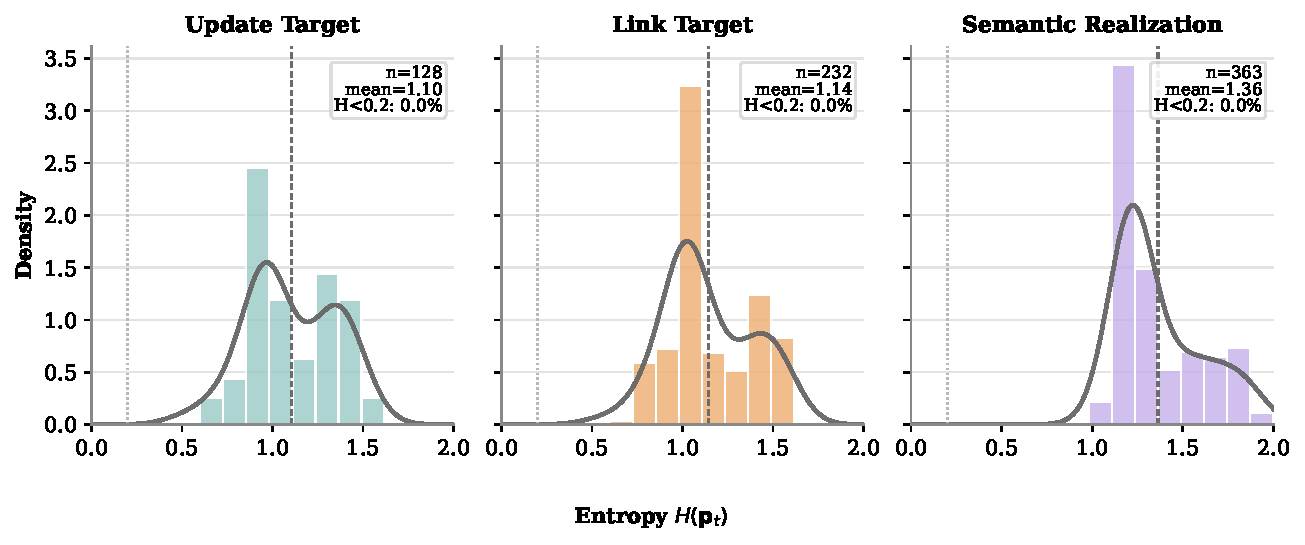
\includegraphics[width=\linewidth]{figures/entropy_histogram.pdf}
\caption{\textbf{Per-carrier entropy of LLM self-reported weights}.
Histograms are shown for \amem{} watermark run on Qwen3.6. All
three carriers place substantial mass away from $H{=}0$, and the
fraction of near-deterministic decisions ($H<0.2$) remains small. This
supports the RQ2 claim that prompted candidate enumeration yields
genuine selection freedom.}
\label{fig:entropy-hist}
\end{figure}


% ============================================================
\subsection{RQ3 — Snapshot-Only / Partial-Log Verification (Headline)}
\label{sec:rq3}
% ============================================================
\paragraph{Motivation.} \todo{In the most forensically valuable
case — memory leaked, distilled, or migrated — the action trace is
gone. RQ1 / RQ2 give ``watermark works at runtime''; this section
gives ``watermark works after the trajectory is gone''. Direct point
of differentiation from action-layer watermarks.}

\paragraph{Regimes.} \todo{R1 = full external log (audit upper
bound). R2 = partial log with keep ratio $r \in \{0.1, 0.3, 0.5,
0.7, 0.9\}$. R3 = snapshot only with the in-record reveal sidecar.}

% ============================================================
% Table: RQ3 verification regime hierarchy
% ============================================================
\begin{table}[t]
\centering
\scriptsize
\setlength{\tabcolsep}{2.5pt}
\resizebox{\columnwidth}{!}{%
\begin{tabular}{p{0.26\textwidth} l c c c c c c}
\toprule
Regime & Method & Bit Recov. & Decode Succ. & FPR & Wrong-Key Acc. & Root Match & Sig Valid \\
\midrule
\multirow{3}{=}{\textbf{R1 — Full External Log}}
  & \memmark{}                    & 1.000 & 1.000 & -- & 0.150 & 1.000 & 1.000 \\
  & \texttt{signed-metadata-only} & 0.000 & 0.000 & -- & 0.000 & 1.000 & 1.000 \\
  & Action-layer @ ToolBench      & -- & -- & -- & -- & -- & -- \\
\midrule
\multirow{3}{=}{\textbf{R2 — Partial Log $r{=}0.5$}}
  & \memmark{}                    & 0.600 & 0.600 & -- & -- & 1.000 & 1.000 \\
  & \texttt{signed-metadata-only} & 0.000 & 0.000 & -- & 0.000 & 1.000 & 1.000 \\
  & Action-layer @ ToolBench      & -- & -- & -- & -- & -- & -- \\
\midrule
\multirow{3}{=}{\textbf{R3 — Snapshot Only (Headline)}}
  & \memmark{}                    & 1.000 & 1.000 & -- & 0.150 & 1.000 & 1.000 \\
  & \texttt{signed-metadata-only} & 0.000 & 0.000 & -- & 0.000 & 1.000 & 1.000 \\
  & Action-layer @ ToolBench      & -- & -- & -- & -- & -- & -- \\
\bottomrule
\end{tabular}%
}
\caption{\textbf{RQ3 — Verification regime hierarchy}. R1 (full
external log), R2 (partial external log, here $r{=}0.5$, full sweep
in Figure~\ref{fig:r2-curve}), R3 (snapshot only — headline).
Wrong-key acceptance reports the rate at which a verifier with the
wrong key still recovers payload bits; expected $\approx 1/K$ for a
sound construction. Action-layer baseline drops to 0 in R3 because
the trajectory is gone.}
\label{tab:verification}
\end{table}


\paragraph{Headline result.} \todo{R3 \texttt{bit\_recovery} reaches
$\approx 1.0$ with \texttt{anchor\_signature\_valid}; wrong-key
control drops to $\approx 1/K$ (random); the
\texttt{signed-metadata-only} ablation drops to 0. R2 degrades
smoothly with $r$ — see Figure~\ref{fig:r2-curve}.}

% ============================================================
% Figure: R2 bit-recovery vs keep ratio (RQ3)
% ============================================================
\begin{figure}[t]
\centering
\fbox{\parbox{0.95\linewidth}{\centering\todo{Line plot: x-axis keep
ratio $r \in [0.1, 0.9]$, y-axis bit\_recovery\_rate. Two lines:
\memmark{} (rises monotonically from $\approx 0.05$ to $\approx
0.95$) and \texttt{signed-metadata-only} (flat at 0). Highlight the
$r{=}0$ R3 result as a star marker at $\sim$1.0 since R3 doesn't
need external log entries.}\\[6pt] \vspace{4cm}}}
\caption{\textbf{R2 — Bit recovery degrades smoothly with external
log retention $r$}. \memmark{} climbs monotonically with $r$;
\texttt{signed-metadata-only} stays at zero because it embeds no
keyed bits. The $r{=}0$ point on the right corresponds to R3
(snapshot-only), where \memmark{} recovers $\approx 1.0$ — the
headline.}
\label{fig:r2-curve}
\end{figure}


% ============================================================
\subsection{RQ4 — Robustness Against Memory-Specific Attacks}
\label{sec:rq4}
% ============================================================
\todo{Nine attacks $\times$ three strengths $(0.1, 0.3, 0.5)$ over
the watermarked snapshot. Report pre / post bit-recovery,
commitment-fail rate, Merkle-proof-fail rate, missing-leaves rate.}

% ============================================================
% Table: RQ4 robustness — 9 attacks × 3 strengths
% Columns: bit_recovery_post / commitment_fail_rate /
%          merkle_proof_fail_rate / missing_leaves_rate
% ============================================================
\begin{table*}[t]
\centering
\small
\setlength{\tabcolsep}{3pt}
\begin{tabular}{ll cccc cccc cccc}
\toprule
& & \multicolumn{4}{c}{Strength $0.1$} & \multicolumn{4}{c}{Strength $0.3$} & \multicolumn{4}{c}{Strength $0.5$} \\
\cmidrule(lr){3-6}\cmidrule(lr){7-10}\cmidrule(lr){11-14}
Category & Attack & {Recov.} & {ComF} & {MerF} & {Miss} & {Recov.} & {ComF} & {MerF} & {Miss} & {Recov.} & {ComF} & {MerF} & {Miss} \\
\midrule
\multirow{5}{*}{Content tamper}
  & manual\_edits        & \todo{}&\todo{}&\todo{}&\todo{} & \todo{}&\todo{}&\todo{}&\todo{} & \todo{}&\todo{}&\todo{}&\todo{} \\
  & paraphrase\_rewrite  & \todo{}&\todo{}&\todo{}&\todo{} & \todo{}&\todo{}&\todo{}&\todo{} & \todo{}&\todo{}&\todo{}&\todo{} \\
  & edge\_relabel        & \todo{}&\todo{}&\todo{}&\todo{} & \todo{}&\todo{}&\todo{}&\todo{} & \todo{}&\todo{}&\todo{}&\todo{} \\
  & subgraph\_reanchor   & \todo{}&\todo{}&\todo{}&\todo{} & \todo{}&\todo{}&\todo{}&\todo{} & \todo{}&\todo{}&\todo{}&\todo{} \\
  & supersession         & \todo{}&\todo{}&\todo{}&\todo{} & \todo{}&\todo{}&\todo{}&\todo{} & \todo{}&\todo{}&\todo{}&\todo{} \\
\midrule
\multirow{4}{*}{Structural}
  & compaction           & \todo{}&\todo{}&\todo{}&\todo{} & \todo{}&\todo{}&\todo{}&\todo{} & \todo{}&\todo{}&\todo{}&\todo{} \\
  & pruning              & \todo{}&\todo{}&\todo{}&\todo{} & \todo{}&\todo{}&\todo{}&\todo{} & \todo{}&\todo{}&\todo{}&\todo{} \\
  & dedup                & \todo{}&\todo{}&\todo{}&\todo{} & \todo{}&\todo{}&\todo{}&\todo{} & \todo{}&\todo{}&\todo{}&\todo{} \\
  & poisoning            & \todo{}&\todo{}&\todo{}&\todo{} & \todo{}&\todo{}&\todo{}&\todo{} & \todo{}&\todo{}&\todo{}&\todo{} \\
\bottomrule
\end{tabular}
\caption{\textbf{RQ4 — Robustness against 9 memory-specific attacks
$\times$ 3 strengths $(0.1, 0.3, 0.5)$}. \textbf{Recov.}{=}post-attack
\texttt{bit\_recovery\_rate}; \textbf{ComF}{=}\texttt{commitment\_fail\_rate}
(catches content tamper); \textbf{MerF}{=}\texttt{merkle\_proof\_fail\_rate};
\textbf{Miss}{=}\texttt{missing\_leaves\_rate} (catches structural
removal). Content-tamper attacks light \textbf{ComF}; structural
attacks light \textbf{Miss}. \textbf{Recov.} measures decoded bits
over surviving leaves and stays high for content tamper because
Method B inclusion proofs are independent per leaf.}
\label{tab:robustness}
\end{table*}


\paragraph{Smooth vs binary signal split.} \todo{Content-tamper
attacks (manual\_edits, paraphrase\_rewrite, edge\_relabel,
subgraph\_reanchor, supersession) trigger
\texttt{commitment\_fail\_rate} proportional to strength. Structural
attacks (pruning, dedup, poisoning, compaction) trigger
\texttt{missing\_leaves\_rate} since the leaf set itself changes
size — see Figure~\ref{fig:attack-signal-split}.}

% ============================================================
% Figure: Attack signal split (RQ4)
% ============================================================
\begin{figure*}[t]
\centering
\fbox{\parbox{0.95\textwidth}{\centering\todo{Two stacked sub-plots:
(a) commitment\_fail\_rate vs strength for 5 content-tamper
attacks, all rise linearly with strength. (b)
missing\_leaves\_rate vs strength for 4 structural attacks, also
linear. Together they show \memmark{} detects \emph{which}
audit layer caught \emph{which} attack — content vs structural —
a single conflated ``tamper detection rate'' would lose this.}
\\[6pt] \vspace{5cm}}}
\caption{\textbf{Attack signal split — content vs structural
tamper}. Content-tamper attacks (manual\_edits, paraphrase\_rewrite,
edge\_relabel, subgraph\_reanchor, supersession) trigger
\texttt{commitment\_fail\_rate} since leaf bytes change in place.
Structural attacks (pruning, dedup, poisoning, compaction) trigger
\texttt{missing\_leaves\_rate} since the leaf set changes size.
Reporting both lets reviewers see exactly which audit layer caught
which attack.}
\label{fig:attack-signal-split}
\end{figure*}


% ============================================================
\subsection{RQ5 — Memory Integrity}
\label{sec:rq5}
% ============================================================
\todo{Question: does watermark introduce dirty memory? Report only
metrics that are computable end-to-end on \locomo{}: overall
snapshot size, per-$\carrier$ carrier-distribution, QA-time
evidence-grounded retrieval recall, write\_failures. No ground-truth
labels in \locomo{} for update / link / merge correctness, so we
don't claim those.}

% ============================================================
% Table: RQ5 integrity (4 metrics actually computed end-to-end)
% ============================================================
\begin{table}[t]
\centering
\scriptsize
\resizebox{0.92\columnwidth}{!}{%
\begin{tabular}{lcccc}
\toprule
Method & Records & Carrier Dist. & Ev. Recall & Write Fail \\
\midrule
\multicolumn{5}{l}{\emph{\amem{} backend}} \\
\quad \texttt{no-watermark}         & 419 & 122:298:421 & 0.660 & 4 \\
\quad \texttt{signed-metadata-only} & 419 & 156:262:424 & 0.552 & 4 \\
\quad \texttt{random-replace}       & 419 & 146:262:429 & 0.563 & 3 \\
\quad \textbf{\memmark}             & 419 & 213:200:426 & 0.585 & 4 \\
\midrule
\multicolumn{5}{l}{\emph{\graphiti{} backend}} \\
\quad \texttt{no-watermark}         & \todo{} & \todo{} & \todo{} & \todo{} \\
\quad \texttt{signed-metadata-only} & \todo{} & \todo{} & \todo{} & \todo{} \\
\quad \texttt{random-replace}       & \todo{} & \todo{} & \todo{} & \todo{} \\
\quad \textbf{\memmark}             & \todo{} & \todo{} & \todo{} & \todo{} \\
\bottomrule
\end{tabular}%
}
\caption{\textbf{RQ5 — Memory integrity (LoCoMo-computable signals
only)}. \textbf{Records}{=}snapshot size; \textbf{Carrier
Dist.}{=}per-$\carrier$ decision count ratio (update : link :
semantic); \textbf{Ev. Recall}{=}QA-time evidence-grounded retrieval
recall (does the rendered context for each QA contain the
question's evidence dia\_ids?); \textbf{Write Fail}{=}memory write
path exception count. LoCoMo does not ship update / link / merge /
delete / stale-memory / temporal ground-truth labels; we therefore
do not report those columns.}
\label{tab:integrity}
\end{table}


% ============================================================
\subsection{RQ6 — Composability with Content Watermark (Appendix)}
\label{sec:rq6}
% ============================================================
\todo{Brief note: three configurations (memory-only / content-only /
both) on the R1 protocol of \S\ref{sec:rq3}. Detail in
Appendix~\ref{app:composability}.}


% ============================================================
% Conclusion — three pillars: utility preserved, R3, watermark.
% ============================================================
\section{Conclusion}
\label{sec:conclusion}

\todo{\memmark{} is a watermark for long-term agent memory
systems that embeds attribution into the memory backend's own
latent evolve decisions. Across \amem{} and \graphiti{} on
\locomo{} we report three findings: utility is preserved within
statistical noise of the unwatermarked baseline (RQ1); snapshot-only
attribution succeeds at bit\_recovery $= 1.00$ versus $0$ for a
signed-metadata baseline (RQ3, headline); the watermark stays
robust under nine memory-lifecycle attacks (RQ4). Code, audit
traces, and benchmarks are released.}

% ============================================================
% Discussion / Limitations
% ============================================================
\section{limitation}
\label{sec:discuss}
\paragraph{Limitations.}
\todo{talk about future work.}

% =================== bibliography ===================
\bibliography{custom}

% =================== appendix ===================
\appendix
% ============================================================
% Appendix
% ============================================================



\section{Full Proofs}
\label{app:proofs}

This appendix collects the technical material that supports the main
paper's central claims but would be too detailed for the main
narrative. We begin with proof sketches for the sampler properties,
then report the composability analysis, hyperparameter sensitivity, and
per-conversation breakdowns referenced in the main text.

\subsection{Proof of Lemma~\ref{lem:dist-preserve}}
The key idea is the standard binning argument underlying
distribution-preserving keyed selection. Integer-quantize
$\probdist$ into $N$ buckets, apply a cyclic shift determined by a
uniform PRF output, and return the candidate whose interval contains
the shifted point. Marginalizing over the uniform shift recovers the
original interval mass for every candidate, so the keyed pick has the
same marginal distribution as $\probdist$.

\subsection{Proof of Lemma~\ref{lem:cascade}}
Distinct internal decisions use distinct context strings and therefore
distinct nonces $\nonceT = \mathrm{PRF}(K, \ctx)$. Under the standard
PRF assumption, these nonces are computationally indistinguishable from
independent random draws to an adversary without the key. The keyed
picks across a cascade of LLM calls therefore behave independently for
verification purposes, and the expected embedding capacity adds across
valid decision points.

\subsection{Proof of Lemma~\ref{lem:backend-invariant}}
This is an immediate corollary of
Lemma~\ref{lem:dist-preserve}. The marginal expression depends only on
the candidate distribution $\probdist$ and the secret key $K$.
Backend-specific implementation details affect how the candidate set is
enumerated, but once $(\candset, \probdist, \ctx)$ is fixed, the
sampling guarantee is backend-agnostic.

\section{Metrics}
\label{app:metrics}

% ============================================================
% Table: Metric definitions (README §9.2)
% ============================================================
\begin{table*}[t]
\centering
\small
\setlength{\tabcolsep}{3.5pt}
\begin{tabular}{p{0.17\linewidth}p{0.29\linewidth}p{0.46\linewidth}}
\toprule
Category & Metric & Definition / Reporting Unit \\
\midrule

Utility
  & \locomo{} F1
  & precision and recall are computed over predicted versus gold answer
    items, and combined as their harmonic mean. \\

  & BLEU-1
  & Unigram precision between the generated answer and the reference
    answer, measuring lexical overlap at the token level. \\

\midrule

Capacity
  & Bits per memory decision
  & Average number of recoverable watermark bits carried by one write,
    update, delete, link, or merge decision. \\

  & Bits per session
  & Total recoverable watermark capacity within one complete conversation
    session. \\

  & Bits per benchmark episode
  & Total recoverable watermark capacity within one benchmark instance. \\

  & Bits per 100 conversation turns
  & Normalized capacity over long-horizon conversations, reported per
    100 turns. \\

  & Average bits per memory write
  & Average number of recoverable bits carried by each committed memory
    write. \\

\midrule

Carrier-level analysis
  & Per-carrier reliability and capacity
  & All watermark reliability and capacity metrics are additionally
    reported for each carrier:
    $\carrier \in
    \{\text{update\_target}, \text{link\_target},
    \text{semantic\_realization}\}$. \\

\midrule

Robustness
  & Commitment verification fail rate
  & Fraction of tampered memory records whose commitment verification
    fails under the anchored commitment root. Reported per attack type
    in \S\ref{sec:rq4}. \\

  & Merkle proof verification fail rate
  & Fraction of tampered memory records whose Merkle inclusion proof fails
    against the anchored Merkle root. Reported per attack type in
    \S\ref{sec:rq4}. \\

\midrule

Memory integrity
  & Snapshot size
  & Total size of the memory snapshot after watermarking and commitment
    construction. \\

  & Carrier distribution
  & Distribution of embedded bits across carriers, reported overall and
    per $\carrier$. \\

  & Evidence-grounded retrieval recall
  & Fraction of QA-time gold evidence records successfully retrieved from
    memory. \\

  & Write failures
  & Number or fraction of attempted memory writes that fail validation,
    storage, or commitment construction. \\

\bottomrule
\end{tabular}
\caption{Metric definitions across the five research questions. Utility
metrics measure answer quality on \locomo{}; watermark metrics measure
decodability, reliability, and security; capacity metrics quantify how many
bits can be carried by memory operations; carrier-level metrics decompose
performance by watermark carrier; tamper-detection metrics measure whether
memory modifications are caught by commitment and Merkle verification; and
memory-integrity metrics measure the operational side effects of watermarking.
For paper-comparability, F1 follows \amem{}'s set-based formula.}
\label{tab:metric-defs}
\end{table*}
Table~\ref{tab:metric-defs} consolidates the definitions of all metrics
used in this paper, grouped by the research question they address: utility
(RQ1), watermark reliability (RQ2), capacity (RQ3), tamper detection (RQ4),
and memory integrity (RQ5). For each metric we list its reporting unit and,
where relevant, the carrier-level decomposition along
$\carrier \in \{\text{update\_target},\ \text{link\_target},\
\text{semantic\_realization}\}$. We refer the reader to this table
throughout Sections~\ref{sec:rq1}--\ref{sec:rq5} for precise definitions.


\section{Composability Experiment}
\label{app:composability}
We evaluate three configurations --- memory-only, content-only, and
both --- under the R1 protocol of \S\ref{sec:rq3}. The purpose is to
check whether memory-level attribution and output-level watermarking
remain operational when deployed simultaneously. We report
(i) memory decode rate, (ii) content watermark detection, and
(iii) joint utility. Table~\ref{tab:composability} summarizes the
comparison.

% ============================================================
% Table: RQ6 composability (appendix)
% ============================================================
\begin{table}[t]
\centering
\small
\setlength{\tabcolsep}{4pt}
\begin{tabular}{lccc}
\toprule
Configuration & Memory Decode & Content Detect & Joint F1 \\
\midrule
memory-only  & \todo{} & N/A     & \todo{} \\
content-only & N/A     & \todo{} & \todo{} \\
both         & \todo{} & \todo{} & \todo{} \\
\bottomrule
\end{tabular}
\caption{\textbf{RQ6 — Composability with content-layer watermark}
on \S\ref{sec:rq3} R1 protocol. Both watermarks coexist without
mutual interference; joint F1 stays within statistical noise of
either standalone.}
\label{tab:composability}
\end{table}


\section{Hyperparameter Sensitivity}
\label{app:hyperparam}
We sweep $K \in \{2, 4, 8\}$ and
$T_{\text{enum}} \in \{0.5, 0.7, 1.0\}$ to quantify the trade-off
between candidate diversity and embedding stability. We report realized
bits per decision together with the corresponding utility deltas, so
that the reader can see how much attribution capacity is obtained per
unit of behavioral perturbation.

% ============================================================
% Table: Hyperparameter sweep (appendix)
% ============================================================
\begin{table}[t]
\centering
\small
\setlength{\tabcolsep}{4pt}
\begin{tabular}{ccccc}
\toprule
$K$ & $T_{\text{enum}}$ & bits/decision & $\Delta$F1 vs no-wm & R3 Recov. \\
\midrule
2 & 0.7 & \todo{} & \todo{} & \todo{} \\
4 & 0.5 & \todo{} & \todo{} & \todo{} \\
4 & 0.7 & \todo{} & \todo{} & \todo{} \\
4 & 1.0 & \todo{} & \todo{} & \todo{} \\
8 & 0.7 & \todo{} & \todo{} & \todo{} \\
\bottomrule
\end{tabular}
\caption{\textbf{Hyperparameter sweep} on candidate count $K$ and
enumeration temperature $T_{\text{enum}}$. $K{=}4, T_{\text{enum}}{=}0.7$
is the default in the main paper.}
\label{tab:hyperparam}
\end{table}


\section{Per-Conversation Breakdown}
\label{app:per-conv}
Finally, we provide the per-conversation breakdown for all
10 \locomo{} conversations. This table is included only in the
appendix because its role is diagnostic rather than conceptual: it
shows that the aggregate trends in the main text are not driven by a
single conversation outlier.

% ============================================================
% Table: Per-conversation breakdown (appendix)
% Auto-generated from individual conv*_metrics_summary.md files.
% ============================================================
\begin{table*}[t]
\centering
\scriptsize
\setlength{\tabcolsep}{3pt}
\begin{tabular}{c c cccc cccc cccc}
\toprule
& & \multicolumn{4}{c}{\amem{}} & \multicolumn{4}{c}{\graphiti{}} & \multicolumn{4}{c}{Watermark Metrics} \\
\cmidrule(lr){3-6}\cmidrule(lr){7-10}\cmidrule(lr){11-14}
Conv & QAs & {F1 wm} & {F1 nwm} & {$\Delta$} & {Ev. R.} & {F1 wm} & {F1 nwm} & {$\Delta$} & {Ev. R.} & {R1} & {R2 $r{=}0.5$} & {R3} & {Wrong K.} \\
\midrule
0 & \todo{} & \todo{} & \todo{} & \todo{} & \todo{} & \todo{} & \todo{} & \todo{} & \todo{} & \todo{} & \todo{} & \todo{} & \todo{} \\
1 & \todo{} & \todo{} & \todo{} & \todo{} & \todo{} & \todo{} & \todo{} & \todo{} & \todo{} & \todo{} & \todo{} & \todo{} & \todo{} \\
2 & \todo{} & \todo{} & \todo{} & \todo{} & \todo{} & \todo{} & \todo{} & \todo{} & \todo{} & \todo{} & \todo{} & \todo{} & \todo{} \\
3 & \todo{} & \todo{} & \todo{} & \todo{} & \todo{} & \todo{} & \todo{} & \todo{} & \todo{} & \todo{} & \todo{} & \todo{} & \todo{} \\
4 & \todo{} & \todo{} & \todo{} & \todo{} & \todo{} & \todo{} & \todo{} & \todo{} & \todo{} & \todo{} & \todo{} & \todo{} & \todo{} \\
5 & \todo{} & \todo{} & \todo{} & \todo{} & \todo{} & \todo{} & \todo{} & \todo{} & \todo{} & \todo{} & \todo{} & \todo{} & \todo{} \\
6 & \todo{} & \todo{} & \todo{} & \todo{} & \todo{} & \todo{} & \todo{} & \todo{} & \todo{} & \todo{} & \todo{} & \todo{} & \todo{} \\
7 & \todo{} & \todo{} & \todo{} & \todo{} & \todo{} & \todo{} & \todo{} & \todo{} & \todo{} & \todo{} & \todo{} & \todo{} & \todo{} \\
8 & \todo{} & \todo{} & \todo{} & \todo{} & \todo{} & \todo{} & \todo{} & \todo{} & \todo{} & \todo{} & \todo{} & \todo{} & \todo{} \\
9 & \todo{} & \todo{} & \todo{} & \todo{} & \todo{} & \todo{} & \todo{} & \todo{} & \todo{} & \todo{} & \todo{} & \todo{} & \todo{} \\
\midrule
\textbf{Mean} & \todo{} & \todo{} & \todo{} & \todo{} & \todo{} & \todo{} & \todo{} & \todo{} & \todo{} & \todo{} & \todo{} & \todo{} & \todo{} \\
\bottomrule
\end{tabular}
\caption{\textbf{Per-conversation breakdown on \locomo{} all 10
samples}. F1 wm / nwm = \memmark{} vs \texttt{no-watermark} F1 (set
formula). Ev. R. = evidence-grounded retrieval recall. Watermark
metrics use the \amem{} backend numbers.}
\label{tab:per-conversation}
\end{table*}



\end{document}
